\input{kapittel}

\kapittel{3}{Eksistens og entydighet}
\label{ch:eksistens-entydighet}

Ved å bruke gausseliminasjon, slik vi snakket om i forrige kapittel,
kan vi løse et hvilket som helst lineært likningssystem på en
strukturert og effektiv måte.  Men det er et par ting vi må tenke på:
Det er ikke sikkert at systemet har noen løsning.  Og om det har
løsning, så er det ikke sikkert at det har bare én løsning -- det kan
ha flere.

Vi skal derfor bruke dette kapitlet på å ta for oss disse to
spørsmålene som vi kan stille om et lineært likningssystem:
\begin{enumerate}
\item Spørsmålet om \emph{eksistens}: Har systemet noen løsning?
\item Spørsmålet om \emph{entydighet}: Hvis systemet har en løsning,
har det kun én løsning, eller flere?
\end{enumerate}

Vi kunne ha spurt om det samme ved å stille bare ett spørsmål:
\emph{Hvor mange løsninger har systemet?}  Men ofte er det mer
praktisk å tenke på eksistens og entydighet som to separate spørsmål.
Noen ganger er vi kun interessert i å vite om et system har løsning
eller ikke, uten å være opptatt av hvor mange løsninger det eventuelt
har.  Andre ganger vet vi at et system har en løsning, men vi er
interessert i å finne ut om den løsningen er den eneste.


\section*{Eksistens}

Her er et lineært likningssystem:
\[
\systeme{
  x + y = 4,
  4x - 2y = 0
}
\]
Vi kan tegne grafene til likningene i systemet:
\begin{center}
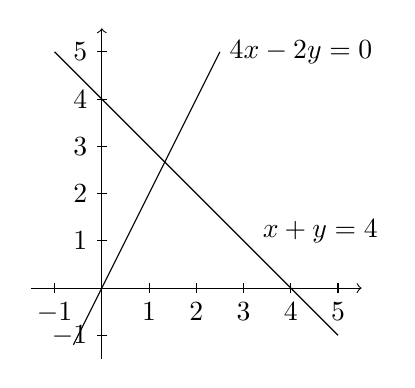
\begin{tikzpicture}[scale=.6]
\draw[->] (-1.5,0) -- (5.5,0);
\draw[->] (0,-1.5) -- (0,5.5);
\foreach \x in {-1,1,2,...,5}
\draw (\x,.1) -- (\x,-.1) node[anchor=north] {$\x$};
\foreach \y in {-1,1,2,...,5}
\draw (.1,\y) -- (-.1,\y) node[anchor=east] {$\y$};
\draw (-1,5) -- (5,-1); % y = 4 - x
\node[anchor=west] at (3.2,1.2) {$x + y = 4$};
\draw (-.6,-1.2) -- (2.5,5) % y = 2x
  node[anchor=west] {$4x - 2y = 0$};
\end{tikzpicture}
\end{center}
Det er tydelig at systemet har en løsning, nemlig der de to grafene
krysser hverandre.

Her er et annet likningssystem:
\[
\systeme{
   x -  2 y = 1,
-5 x + 10 y = -1
}
\]
Grafene til likningene i dette systemet ser slik ut:
\begin{center}
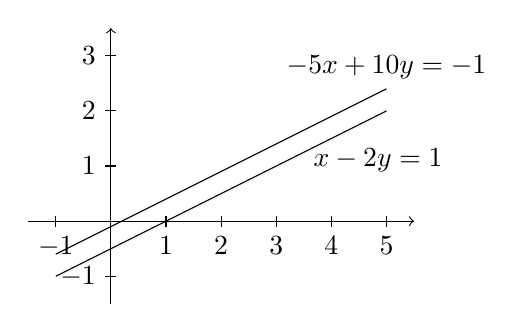
\begin{tikzpicture}[scale=.7]
\draw[->] (-1.5,0) -- (5.5,0);
\draw[->] (0,-1.5) -- (0,3.5);
\foreach \x in {-1,1,2,...,5}
\draw (\x,.1) -- (\x,-.1) node[anchor=north] {$\x$};
\foreach \y in {-1,1,2,...,3}
\draw (.1,\y) -- (-.1,\y) node[anchor=east] {$\y$};
\draw (-1,-1) -- (5,2); % y = x/2 - 1/2
\node[anchor=west] at (3.5,1.1) {$x - 2y = 1$};
\draw (-1,-.6) -- (5,2.4) % y = x/2 - 1/10
  node[anchor=south] {$-5x + 10y = -1$};
\end{tikzpicture}
\end{center}
Nå fikk vi to parallelle linjer som grafer, så de kan aldri krysse
hverandre.  Dermed har dette systemet ingen løsning.

Hvordan ser dette ut når vi forsøker å løse likningssystemet med
gausseliminasjon?  Slik:
\[
\begin{amatrix}{2}
 1 & -2 &  1 \\
-5 & 10 & -1
\end{amatrix}
\roweq
\begin{amatrix}{2}
1 & -2 & 1 \\
0 &  0 & 4
\end{amatrix}
\]
Den siste matrisen svarer til følgende system:
\[
\systeme{
  x + 2 y = 1,
0 x + 0 y = 4
}
\]
Likningen $0x + 0y = 4$ kan også skrives som $0 = 4$, og den kan ikke
stemme uansett hva vi setter $x$ og~$y$ til å være.  Dette systemet
har altså ingen løsning.

Generelt er det slik at hvis vi får en rad i totalmatrisen vår på
formen
\[
0\ 0\ \cdots\ 0\ |\ b,
\]
der $b$ er et tall som ikke er~$0$, så har systemet ingen løsning.
Denne raden svarer jo til likningen $0 = b$, som ikke kan være sann.
Hvis vi har en matrise på trappeform der ingen av radene er på denne
formen, så har systemet minst én løsning.


\section*{Entydighet}

Nå har vi sett eksempler på systemer med én løsning og med ingen
løsning.  Men et lineært likningssystem kan også ha mer enn én
løsning, som vi skal se i det neste eksempelet.

\begin{ex}
\label{ex:gausseliminasjon3}
La oss løse følgende system:
\[
\systeme{
  x_1 + 3 x_2 + 2 x_3 + 3 x_4 = 16,
  x_1 + 3 x_2 + 3 x_3 +   x_4 = 21,
2 x_1 + 6 x_2 + 4 x_3 + 6 x_4 = 32
}
\]
Vi setter opp totalmatrisen og gausseliminerer:
\begin{align*}
\begin{amatrix}{4}
1 & 3 & 2 &  3 & 16 \\
1 & 3 & 3 &  1 & 21 \\
2 & 6 & 4 &  6 & 32
\end{amatrix}
&\roweq
\begin{amatrix}{4}
1 & 3 & 2 &  3 & 16 \\
0 & 0 & 1 & -2 &  5 \\
0 & 0 & 0 &  0 &  0
\end{amatrix}
\\
&\roweq
\begin{amatrix}{4}
1 & 3 & 0 &  7 & 6 \\
0 & 0 & 1 & -2 & 5 \\
0 & 0 & 0 &  0 & 0
\end{amatrix}
\end{align*}
Den siste matrisen svarer til følgende system:
\[
\systeme*{
x_1 + 3 x_2 + 7 x_4 = 6,
x_3 - 2 x_4 = 5
}
\]
(Her har vi ikke tatt med noen likning for nullraden i matrisen.  Det
er fordi nullraden står for likningen $0x_1 + 0x_2 + 0x_3 + 0x_4 = 0$,
eller med andre ord $0 = 0$.  Denne likningen er åpenbart oppfylt
uansett hva $x_1$, $x_2$, $x_3$ og~$x_4$ er, så vi trenger ikke ta den
med.)

Hvis vi flytter alt unntatt $x_1$ og~$x_3$ til høyresiden, ser
systemet slik ut:
\[
\left\{
\begin{aligned}
x_1 &= - 3 x_2 - 7 x_4 + 6 \\
x_3 &= 2 x_4 + 5
\end{aligned}
\right.
\]
Vi kan altså finne løsninger av systemet ved å sette $x_2$ og~$x_4$
til å være hva vi vil, og deretter bruke disse to likhetene til å
bestemme $x_1$ og~$x_3$.

Hvis vi for eksempel velger $x_2 = 0$ og $x_4 = 1$, så får vi
følgende løsning:
\[
\left\{
\begin{aligned}
x_1 &= -3 \cdot 0 - 7 \cdot 1 + 6 = -1 \\
x_2 &= 0 \\
x_3 &= 2 \cdot 1 + 5 = 7 \\
x_4 &= 1
\end{aligned}
\right.
\]

For å beskrive alle løsningene av systemet på en ryddig måte, kan vi
sette $x_2 = s$ og $x_4 = t$, der $s$ og~$t$ står for to vilkårlige
tall.  Da er alle løsningene gitt ved:
\[
\raisebox{23pt}{$
\left\{
\begin{aligned}
x_1 &= -3 s - 7 t + 6 \\
x_2 &= s \\
x_3 &= 2 t + 5 \\
x_4 &= t
\end{aligned}
\right.
$}
\qedhere
\]
\end{ex}

Variabler som vi kan sette til hva vi vil, slik som $x_2$ og~$x_4$ i
eksempelet over, kalles \defterm{frie variabler}.


\section*{Tre muligheter}

Nå har vi sett eksempler på alle muligheter som finnes for antall
løsninger av et lineært likningssystem.  La oss oppsummere.

Det kan hende at vi, når vi gausseliminerer, får en rad som har et
pivotelement til høyre for streken.  Den raden tilsvarer en umulig
likning, og dermed har systemet ingen løsning.

Hvis vi har gausseliminert helt til trappeform og alle pivotelementene
holder seg til venstre for streken, så har systemet løsning.  Da kan
det hende at vi får en fri variabel (eller flere), og i så fall er det
uendelig mange løsninger.  Eller så blir det ikke noen fri variabel,
og da har systemet nøyaktig én løsning.

Men det som ikke under noen omstendighet kan skje, er at vi får
nøyaktig to løsninger, eller tre løsninger, eller nitten eller
trettisju eller femhundreogsekstito løsninger.

Og her skiller lineære systemer seg markant ut fra det vi vet om
likningssystemer generelt.  Det er jo ikke noe problem å finne en
likning som har mer enn én løsning, men ikke uendelig mange.  Se for
eksempel på noe så enkelt som likningen $x^2 - 9 = 0$: Den har to
løsninger ($3$ og~$-3$).  Så snart vi har med noe ikkelineært i
systemet vårt, er det altså fullt mulig å få nøyaktig to løsninger,
eller fjorten, eller nittiåtte.  Men med bare lineære likninger går
det ikke an -- da har vi bare disse tre mulighetene:
\begin{enumerate}
\item Systemet har ingen løsning.
\item Systemet har entydig løsning.
\item Systemet har uendelig mange løsninger.
\end{enumerate}


\section*{Valgfrihet}

Når vi gausseliminerer har vi en viss grad av valgfrihet.  Det som
står fast er hva vi har lov til å gjøre, nemlig de tre typene
radoperasjoner, og hva vi vil ende opp med, nemlig (redusert)
trappeform.  Nøyaktig hvordan vi bruker radoperasjoner for å komme
frem kan vi velge selv.

Vi tar et enkelt eksempel for å illustrere dette.

\begin{ex}
Anta at vi vil gausseliminere denne totalmatrisen:
\[
\begin{amatrix}{4}
0 & 2 & 4 & 1 & 7 \\
3 & 8 & 2 & 0 & 4 \\
5 & 9 & 2 & 4 & 4
\end{amatrix}
\]
Her er vi nødt til å bytte øverste rad med en av de to andre for å få
pivotelementet i første rad på riktig sted.  Men vi velger selv
hvilken av de to radene vi vil flytte til toppen.
\end{ex}

Vi har også noe frihet når det gjelder valg av frie variabler.

\begin{ex}
I eksempel~\ref{ex:gausseliminasjon3} endte vi opp med at de to
variablene $x_2$ og~$x_4$ var frie.  Men vi kunne også ha valgt å la
$x_1$ og~$x_3$ være frie, som vi skal se nå.

Vi hadde forenklet systemet til følgende:
\[
\left\{
\begin{aligned}
x_1 &= - 3 x_2 - 7 x_4 + 6 \\
x_3 &= 2 x_4 + 5
\end{aligned}
\right.
\]
Vi kan løse den andre likningen her for~$x_4$ og få:
\[
x_4 = \frac{x_3 - 5}{2}
%\frac{1}{2} x_3 - \frac{5}{2}
\]
Deretter kan vi sette inn dette i den første likningen og løse
for~$x_2$:
\begin{align*}
x_2
&= \frac{- x_1 - 7 x_4 + 6}{3} \\
&= \frac{- x_1 - \frac{7}{2} (x_3 - 5) + 6}{3} \\
&= - \frac{1}{3} x_1 - \frac{7}{6} x_3 + \frac{47}{6}
\end{align*}
Hvis vi nå lar $x_1 = s$ og $x_3 = t$, så har vi følgende generelle
løsning:
\[
\left\{
\begin{aligned}
x_1 &= s \\
x_2 &= - \frac{1}{3} s - \frac{7}{6} t + \frac{47}{6} \\
x_3 &= t \\
x_4 &= \frac{1}{2} x_3 - \frac{5}{2}
\end{aligned}
\right.
\]
Dette ser annerledes ut enn det vi fikk i
eksempel~\ref{ex:gausseliminasjon3}, men det beskriver nøyaktig de
samme løsningene.  (Du kan for eksempel sjekke at hvis vi her setter
$s=-1$ og~$t=7$, så får vi den samme løsningen som da vi valgte
$x_2=0$ og~$x_4=1$ i eksempel~\ref{ex:gausseliminasjon3}).
\end{ex}


\kapittelslutt
